\section{Introduction}
\subsection{Motivation}
In the space of \ac{HPC}, a significant trend from more compute-intensive tasks to more data-intensive tasks is taking place. This change necessitates better data-management tooling such as data lakes or data warehouses. Given that \ac{HPC} computes on raw data, data lakes are a more natural fit. Efficient metadata management requires a great metadata store as well as support for full-text searches.

In this report, the viability of Elasticsearch\footnote{\url{https://www.elastic.co/elasticsearch}} for \ac{HPC} load is being evaluated. Elasticsearch benefits from many years of tooling development, making it a more pragmatic choice than building an own application around full-text search engines like Apache Lucene\footnote{\url{https://lucene.apache.org/}} or Tantivy\footnote{\url{https://github.com/quickwit-oss/tantivy}}.

While elastic provides rally\footnote{\url{https://github.com/elastic/rally}}, an in-house benchmark suite used for performance regression testing \cite{es_benchmarking}, after rigorous internal testing it was found out that thespian\footnote{\url{https://thespianpy.com/doc/}}, its internal actor framework, did not scale up to more than 60 nodes, which was not sufficient for previous large-scale stress testing. Thus, for this report a new benchmarking framework was designed, using reliable \ac{HPC} native technologies such as \ac{MPI}.

In addition, the data lake related use cases at the GWDG include spawning Elasticsearch instances on-demand. For this dynamic deployment, a containerized Elasticsearch cluster based on the underlying \ac{SLURM}\footnote{\url{https://slurm.schedmd.com/documentation.html}} and \ac{MPI} are needed. It should auto-configure itself, in order to be IP-agnostic.
\subsection{Goals and Contributions}
The goals of this report are twofold: First, providing and implementing a stateful architecture to dynamically spawn and respawn an Elasticsearch cluster without any previous manual configuration. Second, design a highly-scalable, \ac{HPC}-native, distributed Elasticsearch benchmarking framework for both ingestion and querying performance. 

To achieve these goals, the following contributions were made:

\begin{itemize}
\item Design and implementation of a zero-configuration workflow to spawn a rootless, containerized Elasticsearch cluster of arbitrary size within a SLURM-allocated \ac{MPI} environment.
\item Design and implementation of a highly scalable, distributed benchmarker for ingestion performance
\item Design and implementation of a highly scalable, distributed benchmarker for query performance with custom benchmark scenarios using a \ac{JSON}-based \ac{DSL}.
\item Benchmark a dynamically spawned Elasticsearch cluster on \ac{HPC} using a canonical dataset common in existing literature.
\end{itemize}
\subsection{Structure}
This report is structured as follows: In section 2, Elasticsearch, the full-text search engine and NoSQL database used, is introduced. After that, section 3 covers the related work starting with classical load generation before focussing on the literature around Elasticsearch benchmarking. In section 4, the methodology and design of all components are covered. First, it covers the design and internal workflow of the aforementioned cluster spawning mechanism. Then, it covers both the ingestion and query benchmarkers. Lastly, it focuses on the benchmark design by showing the steps required to perform the benchmarks and the reasoning behind the corpus and query design used in this specific benchmark. Lastly, in section 5 the results of the benchmark are shown, before describing the open problems and challenges in Chapter 6. Concluding in Chapter 7, the results are summarized and possible future work is shown.

\section{Background}
\subsection{Elasticsearch}
Elasticsearch is a distributed search engine initially developed in 2010. Since it stores its data in a document model, it can also be seen as a NoSQL database. The full-text search internally relies on the Apache Lucene library. It is mainly used for its full-text fuzzy search capabilities and its \ac{JSON}-based REST interface. It is used by many large websites such as Wikipedia\footnote{Wikipedia also used Lucene beforehand.}, Netflix, Stackoverflow, and LinkedIn.

In Elasticsearch, a collection of \emph{documents} are stored in an \emph{index}. Documents are equivalent to, and can be sent in the form of, \ac{JSON} objects. They can be nested. Each index has a \emph{schema}, which is a type mapping for each of the key-value pairs contained in the index\footnote{Akin to a SQL database definition.}. This mapping can either be statically preconfigured or dynamically guessed at ingestion time. The index data can be \emph{queried} using Elasticsearchs own \ac{DSL}, again relying on \ac{JSON} and REST as the foundational technology.

In 2021, due to a license change from Apache 2.0 to a more permissive license, OpenSearch was created as an Elasticsearch fork, which is maintained by several companies such as AWS.

\section{Related Work}
While the topic of Elasticsearch benchmarking is more sparsely covered, a lot of previous work around general HTTP API benchmarking exists. The most used load generator is Apache JMeter \cite{jmeter}, a sophisticated graphical load tester that supports many protocols such as HTTP(S), SOAP, or LDAP. Only relying on the \ac{CLI} interface, wrk \cite{wrk} provides a simpler popular alternative. For a more scriptable alternative, the Javascript-based Grafana k6 \cite{k6} gained a lot of popularity over recent years.\\

For benchmarking Elasticsearch, the main tool is the aforementioned rally \cite{rally}, a microbenchmarking framework developed by Elastic. While it can be run on a single node, it also supports distributed benchmarking through the Thespian actor system.

Different benchmarking scenarios are defined as so-called \emph{tracks}. Every track contains one or more \emph{corpora}, containing \ac{NDJSON} objects as documents. All tracks are available on GitHub \cite{rallytracks}. Each track contains many \emph{operations} such as ingestion or specific queries, which are then structured into a \emph{challenge's} \emph{schedule} in a fork-join model. This means that Rally can be extended without editing the source code.

The rally framework is actively used in literature for benchmarking Elasticsearch clusters \cite{rallyusecase1} \cite{rallyusecase2} \cite{rallyusecase3}. As mentioned in the introduction, it was not a viable choice for this paper due to the underlying actor framework not scaling into more than 128 nodes in previous experiments.

Furthermore, most of the benchmark comparisons between NoSQL databases such as tsbs \cite{tsbs} are done by database vendors themselves, resulting in conflicting financial interests.

\section{Methodology and Design}
The Methodology and Design section is split into four parts: First, the autoconfigured Elasticsearch cluster spawner is presented. After that, the next two subsections cover the distributed ingestion and query benchmarker respectively, including underlying reasoning as well as some technical details. Lastly, the overall benchmark design used for this report is discussed, focusing mainly on the high-level benchmark workflow as well as the corpus and query design.

\subsection{Dynamic Cluster Creation Based on MPI Communicator}
This section presents an automated approach to configuring and spawning a multi-node Elasticsearch cluster based solely on the \ac{MPI} environment set up by SLURM. It dynamically fetches the different hosts, i.e. it is not required to know the hostnames or IPs beforehand, making it easily embeddable in any kind of job system. The cluster is very portable since it is using Singularity \cite{singularity} containers as an Elasticsearch host. Any cluster size larger or equal to two nodes is supported. The code can be found on GitHub \cite{myspawner}.

Furthermore, it supports \emph{statefulness}, which means that the same cluster can be re-spawned on other nodes\footnote{With the same cluster size.} without requiring a re-ingest, i.e. keeping the complete cluster state and configuration. Due to the aforementioned containerization, this also works while changing both the hardware and IP addresses. The only limitation is that it only supports one Elasticsearch node per host OS. This is by design, as we use hostname-based resolution instead of IP-based resolution to be agnostic to the \ac{NIC} used\footnote{Being \ac{NIC} agnostic implies that it supports both ethernet and InfiniBand.}. 

This automatic containerization has the big advantage that it can be embedded into any kind of job pipeline. While most web services require a continuously running search engine, it is common in \ac{HPC} that applications are spawned on demand only when needed and torn down once the computation is performed. More importantly, it allows for Elasticsearch to be implicitly spawned as a dependency for other, more cloud-native applications running in \ac{HPC}.\\

The high-level idea is as follows: For discovery and information communication, \ac{MPI} is used. Furthermore, based on the world size, the number of master eligible nodes is decided\footnote{If $N \leq 3$ then 1 master eligible node, otherwise 3 master eligible nodes. Note that only one master is active at a time. An odd number was chosen to prevent a split brain.}. After that, each node creates a config and runtime environment for itself. Lastly, each process spawns its container using its newly generated config.\\

For better portability and reproducibility, the cluster generator uses Singularity containers internally\footnote{Note that, due to Elasticsearch JDK problems, Singularity has to be started with \texttt{-{}-cleanenv}. Therefore environment variables get ignored within the container.}. The container is based on the official Ubuntu 22.04 docker image\footnote{\url{https://hub.docker.com/_/ubuntu}}, only adding packages for debugging and maintenance. Elasticsearch itself is not part of the image and is completely bind-mounted in; there are multiple reasons for this: First, unlike docker, Singularity containers are always immutable, so the program state itself has to always be bind-mounted in. Furthermore, Elasticsearch expects to be the owner of its folders. If Elasticsearch is not the folder owner, it disables multiple features such as internal auto-configuration. Since Singularity is rootless, the correct uid for the folders can't be enforced. Therefore, the most straightforward and stable solution is bind-mounting it in.\\

The workflow has the following steps:
\begin{itemize}
  \item First, check if the Elasticsearch index data from the last run can be reused. This is the case if the number of nodes stayed the same. If not, create a new Elasticsearch into a temporary directory.
  \item \texttt{MPI\_GATHER} a list of tuples \texttt{(rank, hostname)} into the root rank 0.
  \item For each node, the root creates/updates the config; the other nodes are waiting. Note that through updating the config instead of creating a new one the cluster stays intact, which is how the statefulness is implemented. An example config can be found in the appendix.
  \item Lastly, each rank starts the immutable singularity container with the new config and previously created Elasticsearch mounted in.
\end{itemize}

\newpage

\subsection{Distributed Ingestion Benchmarker}
This section introduces the distributed, \ac{MPI}-based ingestion benchmarker \cite{myingestion}. It is used both for providing a fast way to ingest a \ac{JSON}-formatted corpus into an Elasticsearch cluster as well as measuring the performance of write operations in throughput as well as latency. The benchmarker itself is very I/O optimized, using so-called offset caching for reducing redundant operations between workers. It supports statically typed index definitions, configurable bulk size as well as a configurable number of shards. It supports all corpora designed for Elastic's rally benchmarker by using \ac{NDJSON} as an input format\footnote{Another big advantage of \ac{NDJSON} is that downscaling the benchmark is trivial using\\\texttt{head -n <NEW\_NUMBER> original.json > downscaled.json}}. The \ac{CLI} interface with all its features can be found in the appendix.\\

The benchmark can be split into three phases:

\paragraph{Setup:}
Note that those steps are done by only the root/rank 0.
\begin{itemize}
  \item Create the offset cache.

    The offset cache is needed for the following reason: To do the ingestion in a distributed manner, the bulk ingest load has to be split evenly between all nodes. This is done by giving each rank (approximately) the same number of documents in the corpus file. Note that \ac{NDJSON} implies one document per line. For $N$ nodes and $L$ lines, each rank $i$ gets the range
    \[
      \left[ \frac{i}{N} \cdot L, \frac{i+1}{N} \cdot L \right)
    \]
    But this requires that the number of lines have to be known, which implies reading the whole file at least once. After the range has been computed, the file has to be read a second time to find the starting byte to seek to. This is needed since the \ac{JSON} documents have a variadic size in bytes; one can't just compute the $i$-th document through $doc\_size \cdot i$.

    The corpora are often huge; the \texttt{nyc\_taxis} corpus used in this report is around 75GB in size with over 160,000,000 documents. This would create a lot of I/O load if every node would do this every time the benchmark runs.

    So instead, the root computes all offsets once and saves it into a \texttt{.offsets.json} file, which can be reused in future benchmarks, removing all redundant work. This optimization is possible whenever the number of load generators stays the same.

    On a technical level, this is done as follows:
    \begin{enumerate}
      \item Iteration 1: Count the number of lines.
      \item Compute the starting and ending line for each rank using the total number of lines.
      \item Iteration 2: Find the byte offsets for each rank.
      \item Save everything into a \texttt{.offsets.json} file.
      \item Validate that, starting at the current byte, the line of each rank has a complete \ac{JSON} document.
    \end{enumerate}
    An example \texttt{.offsets.json} file can be found in the appendix.

  \item Create an (empty) Elasticsearch index. It is created using the following settings:
    \begin{itemize}
      \item Strict type mappings for reproducibility. Elasticsearch allows for dynamic schemas, which means that the datatype is interpreted when the first data arrives. When using a distributed benchmarker, it is not clear which rank sends the first bulk ingest request. Thus, indeterministic or unexpected behaviour could occur. So instead, using Elasticsearchs own type system\footnote{\url{https://www.elastic.co/guide/en/elasticsearch/reference/current/mapping-types.html}} and \ac{DSL}\footnote{\url{https://www.elastic.co/guide/en/elasticsearch/reference/current/mapping.html}} the type mapping can be defined statically and used by the benchmarker.
      \item The number of shards is explicitly set, defaulting to one shard per Elasticsearch node. This means that every node gets data while still keeping the sharding complexity as trivial as possible. This is configurable via the \ac{CLI} interface.
      \item Explicitly disable caching through \texttt{requests.cache.enable}\footnote{\url{https://www.elastic.co/guide/en/elasticsearch/reference/current/shard-request-cache.html}}
    \end{itemize}
\end{itemize}
At the end of the setup phase, the offsets are sent to all workers using \texttt{MPI\_BROADCAST}.

\paragraph{Benchmark:} This work is done by each rank including the root.
\begin{itemize}
  \item Each rank computes to which Elasticsearch node it should send the data. 

    It is assumed that the user understands that this distribution is a problem that has to be solved. Thus, it is expected that the \ac{MPI} world size is a multiple of the number of Elasticsearch cluster nodes\footnote{It also works when this isn't the case, although the distribution is less optimal.}. With that in mind, the distribution is calculated by \texttt{rank \% N} with \texttt{\%} being the modulo operation and \texttt{N} the number of Elasticsearch cluster nodes

  \item Next, seek to the starting byte based on the rank.
  \item Create and send the requests blockingly, as fast as possible. Track each response time.

    The requests are sent in bulk using Elasticsearches Bulk API\footnote{\url{https://www.elastic.co/guide/en/elasticsearch/reference/current/docs-bulk.html}} with a default bulk size of 1000 documents, configurable via CLI parameter.

    The measurements are done with utmost care to be as precise as possible and minimize the overhead created by the benchmarker itself. Thus, the delta recorded only measures the time directly before and after the HTTP request, removing the query-building overhead.
  \item Once all data is sent, the workers wait at an \ac{MPI} barrier for the other workers to finish.
  \item In the end, all data is gathered at the root process.
\end{itemize}

\paragraph{Teardown:}
Once the data is gathered, the root dumps it into a \ac{JSON} file.

\subsection{Distributed Query Benchmarker}
While the last section focused on the ingestion (write) performance, this section will focus on benchmarking the query (read) performance of an Elasticsearch cluster \cite{myquery}. The benchmarker also generates its load in a distributed manner using the \ac{MPI} environment provided by SLURM. It measures the documents per second as well as the request latency of a cluster when put under load. The benchmark is structured using a fork-join-like model. 

The distributed query benchmarker has the following features:
\begin{itemize}
  \item Fully configurable by a \ac{DSL}-like \ac{JSON} standard; no hard-coded scenarios.

    The \ac{DSL} embeds the Elasticsearch query language internally, making it very accessible to all Elasticsearch users. Furthermore, this allows for extending the benchmarking scenarios without the need to edit the source code. Since the language is a simplification of rally's \ac{DSL}, elastics official benchmarks can be ported easily. An example of a ported rally benchmark can be found in the accompanying repository.

    Also, an example input file using the custom \ac{DSL} can be found in the appendix.
  \item Measuring raw performance by bypassing the cache\footnote{\url{https://www.elastic.co/guide/en/elasticsearch/reference/current/shard-request-cache.html\#_enabling_and_disabling_caching_per_request}}.
  \item Supporting a test mode for verifying the correctness of custom benchmarks.
  \item Parsing the Elasticsearch response instead of just relying on the HTTP response like a normal HTTP benchmarker. This is done to count the number of returned documents.
  \item Supporting multiple, alternating queries in a single fork-join task for creating a more realistic load.
\end{itemize}

On a technical level, each benchmark starts with the following preparation.
\begin{itemize}
  \item First, all \ac{CLI} arguments and the benchmark description are parsed. The benchmark description is written in the aforementioned, JSON-based custom DSL with the Elasticsearch Search API Syntax embedded into it. An example query benchmark description as well as the \ac{CLI} interface structure of both benchmarkers can be found in the appendix.
  \item After that, every rank calculates which Elasticsearch server it sends its load to. See the ingest benchmarker section for a more detailed description of how this selection algorithm works.
\end{itemize}

Once all ranks are ready, the actual benchmark starts. For each of the fully disjunct benchmark steps, the following actions are performed:
\begin{itemize}
  \item First, the root node, i.e. \ac{MPI} rank 0, waits for the Elasticsearch cluster health\footnote{\url{https://www.elastic.co/guide/en/elasticsearch/reference/current/cluster-health.html}} to be green while the other nodes wait at an \ac{MPI} barrier, ready to benchmark. This is done in case the data was just ingested or the cluster was just started on-demand.
  \item As mentioned above, each benchmark step can contain multiple queries, which will then be executed in an alternating manner to simulate a more varied load on the server. Since all ranks start executing the queries at the same time, all ranks might be in sync, sending the exact same query at the same time, which would not be a realistic load. To prevent this, each rank creates a random permutation of all queries for this step.
  \item If the warmup time is set:
    \begin{itemize}
      \item Send the next query, and throw away the result. This is needed to get the caches filled before starting the measurements; therefore reducing the variance of the result data. The index is configured to not do any caching on an Elasticsearch level, however, the OS will still do caching, both on a CPU L1/L2/L3 level as well as I/O caching through the page and buffer cache.
      \item Sleep between results if a waiting time is configured.
    \end{itemize}
  \item Once the warmup is done, the following steps are done until the configured execution time is reached:
    \begin{itemize}
      \item Select the next query.
      \item Track the current time right before sending the request.
      \item Do the request containing the query against the search API endpoint. Note that the cache is explicitly disabled, both on an index level and on a request level\footnote{\url{https://www.elastic.co/guide/en/elasticsearch/reference/current/shard-request-cache.html\#_enabling_and_disabling_caching_per_request}}.
      \item Track the time right after the response was received, before processing the result. This is done for two reasons: First, it minimizes the measurement overhead created by the benchmarker itself and isolates the time Elasticsearch needed for creating and sending the response. Second, it increases the likelihood of our operation being atomic, i.e. that the OS scheduler will not preempt the process by giving the CPU time to another process before the measurement is finished.
      \item Next, it will process and record the result based on the HTTP response code. If it was successful\footnote{i.e. a 2xx HTTP response code}, it will count the number of received documents and will save a tuple \texttt{(latency, docs count)} for the current query and rank. If the request is unsuccessful, it saves the HTTP code for the current query and rank. Note that this all happens in Memory, no slow I/O is done to minimize the benchmarker overhead.
      \item Lastly, sleep between results if a waiting time is configured.
    \end{itemize}
\end{itemize}

Once all measurements are created, the results of all ranks get merged at the root using \ac{MPI} gather as well as some data transformation. The resulting output format can be seen in the appendix. To finish the execution, the root dumps the JSON-formatted results at a path specified via a \ac{CLI} parameter.

\subsubsection{Test Mode}
Designing a database benchmark is complicated; it should be very clear both what the expected result is and whether the query actually produces that result. To verify the correctness of a given benchmark, a test mode was developed. This test mode can be run with \texttt{-{}-test-mode}.

The purpose of the test mode is to give a short overview to check whether the raw Elasticsearch responses contain the results expected. Therefore it is sufficient that the test mode only runs on the root rank. The test mode itself is pretty trivial: It goes through each benchmark step, runs each query once, verifies that the response code is successful, and then prints the request input as well as the response output as prettified JSON into the terminal for further manual inspection.

While designing several benchmarks, it helped finding broken queries generating empty responses.

\subsection{Benchmark Design}
\subsubsection{High-Level Benchmark Workflow}
To create and run a benchmark, the following steps have to be done:
\begin{enumerate}
  \item Choose a dataset or create a synthetic one. The dataset has to be formatted in the \ac{NDJSON} format, which is defined as one JSON object per line. Datasets for many common Elasticsearch use cases can be found in Elastic's rally-tracks repository \cite{rallytracks}.
  \item Define the data type mappings for each corpus attribute using the Elasticsearch index mapping syntax\footnote{\url{https://www.elastic.co/guide/en/elasticsearch/reference/current/properties.html}}. An example can be found in the repository.
  \item Design the query document. This basically consists of embedding the Elasticsearch search API queries into a bigger JSON structure defining the benchmark steps.  Note that the queries themselves do not have to be altered, thus they can also easily be constructed using cURL. Since Elastics rally also uses the search API syntax, their benchmarks can easily be ported. For each benchmark step, the warmup time, execution time, and sleep time between each request can be defined optionally. The query document format can be found in the appendix, and a ported benchmark from rally can be found in the repository.
  \item Spawn up the automatically configured Elasticsearch cluster using the \ac{MPI}-based cluster creator in a given SLURM environment using \texttt{mpirun}. 

    Note that Elasticsearch requires a non-standard Kernel parameter to be set, a \texttt{vm.max\_map\_count} of at least 262144. This setting defines the maximum number of memory map areas per process. This is needed because Elasticsearch accesses the index data by mapping the files into memory using their so-called \texttt{mmapfs}\footnote{\url{https://www.elastic.co/guide/en/elasticsearch/reference/current/vm-max-map-count.html}}, based on Lucenes \texttt{MMapDirectory}\footnote{\url{https://lucene.apache.org/core/6_3_0/core/org/apache/lucene/store/MMapDirectory.html}}.
  \item Run the distributed ingest benchmarker with the previously created corpus and type mapping using \texttt{mpirun}.
  \item Run the distributed query benchmarker with the previously created query document using \texttt{mpirun}.
  \item Analyze all results. A Jupyter notebook in the repository can be used as a starting point.
\end{enumerate}

\subsubsection{Corpus and Query Design}
The benchmark created for this report is a port of rallys \texttt{nyc\_taxis} track \cite{nyctaxis}. Its corpus contains New York taxi data, more specifically all rides that have been performed in yellow taxis in New York in 2015. This data gets published every year by the NYC Taxi and Limousine Commission and can be freely downloaded \cite{tlcdata}. An example corpus document can be found in the appendix.\\

This benchmark was chosen as it is one of the two rally benchmarks most often used in literature, \texttt{geonames}, and \texttt{nyc\_taxis}. In the literature, both of these benchmarks have a specific purpose. 

\paragraph{\texttt{nyc\_taxis}} is mainly used as a scaling test because of its big corpus size with over 165 million documents and comparatively big document size. The documents are very numeric, which makes the data set great for benchmarking range queries and aggregations such as histograms. It can't be used for thorough benchmarking of string-matching capabilities.

\paragraph{\texttt{geonames}} is mostly used as a regression test for various features. It has a very balanced document structure, containing text, keywords, numbers, as well as geolocations. The main advantage of \texttt{geonames} is the number of queries designed for it, including text and keyword matching, several aggregations, scroll API, Elasticsearch's expression and painless scripting languages, and many more niche features of Elasticsearch.

Since the internal use case at the GWDG is mainly around fuzzy matching and range queries running on large corpora in an \ac{HPC} environment, the \texttt{nyc\_taxis} track is a better fit.\\


For the measurements done in this report, a full query benchmark was designed, loosely based on the one provided by Elastic. Note that the main purpose of this benchmark is to provide a starting point on how to design Elasticsearch queries for this benchmarker. 

It contains the following benchmark steps:
\begin{itemize}
  \item Simple, non-filtering \texttt{match\_all}\footnote{\url{https://www.elastic.co/guide/en/elasticsearch/reference/current/query-dsl-match-all-query.html}} requests, with response sizes of 10, 100, 1000, or 10000 documents. This is done to benchmark the base I/O performance and response size scaling.
  \item Next a \texttt{range} query\footnote{\url{https://www.elastic.co/guide/en/elasticsearch/reference/current/query-dsl-range-query.html}}, again scaling up the number of documents between each step. The range query is the exact same one also used by Rally.
  \item After that, it alternates the \texttt{range} and \texttt{match\_all} query in the same benchmark step. This is done to simulate a more varied and realistic load.
  \item In order to measure the latency change given less load, the \texttt{match\_all} query gets executed with 0.02, 0.05, 0.1, 0.2, 0.5, and 1-second sleep between each request.
  \item Lastly, multiple histogram aggregations, either with automatic or manual bucketing, are being executed, all designed by Elastic. This allows us to measure aggregation performance while also being comparable to other benchmarks made with Rally.
\end{itemize}

\section{Test Run and Analysis}
In this section, an example benchmark is shown in order to confirm that works as expected as well as show how this benchmarker could possibly be used in a real scientific benchmarking scenario. This section will be split into three parts: The setup, ingestion results, and query results. Note that all raw data as well as the analysis scripts can be found in the accompanying GitHub repository.

\subsection{Setup}
The aforementioned ported \texttt{nyc\_taxis} benchmark was run on the Emmy\footnote{\url{https://gwdg.de/hpc/systems/emmy/}} supercomputer using 3 dedicated standard96 partition compute nodes to create a 3 node Elasticsearch cluster. The nodes communicated using an ethernet interconnect instead of Intel Omni-Path, although both were tested to work properly. The Singularity container is based on the Ubuntu 22.04 dockerhub image. It runs Elasticsearch 8.11.0, which shipps its own OpenJDK 21.0.1. Elasticsearch indices were configured to not cache at all. The benchmarker used Python 3.9 as well as OpenMPI 4.1.

Note that for these benchmarks a slightly modified version of this benchmarker was used. The main difference was that the benchmarker provided in this report does not support to run the cluster spawner and benchmarker on the same server since both expect to use \texttt{MPI\_COMM\_WORLD}. But for the purposes of this example benchmark, in order to save computing resources, it is okay to execute the load generators and to-be-benchmarked process on the same machine.

\subsection{Ingestion}
For the ingestion benchmarks, the 3 node cluster was ingested with different processes per node (ppn); A ppn of 4 means that for 3 Elasticsearch nodes $3 \cdot 4 = 12$ load generators were spawned. Note that the load generators choose a random Elasticsearch instance to send the data to. This is good, because it imitates the network overhead of a real benchmark.

Here are the results:
\begin{figure}[H]%
    \centering
    \subfloat[\centering {}]{{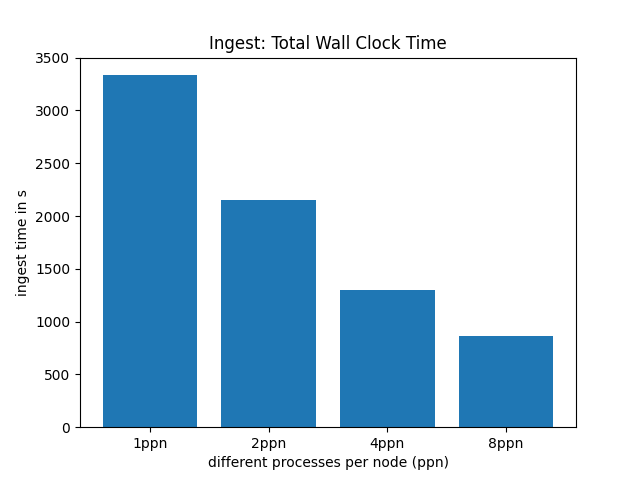
\includegraphics[width=0.45\textwidth]{./analysis/wallclocktime.png} }}%
    \qquad
    \subfloat[\centering {}]{{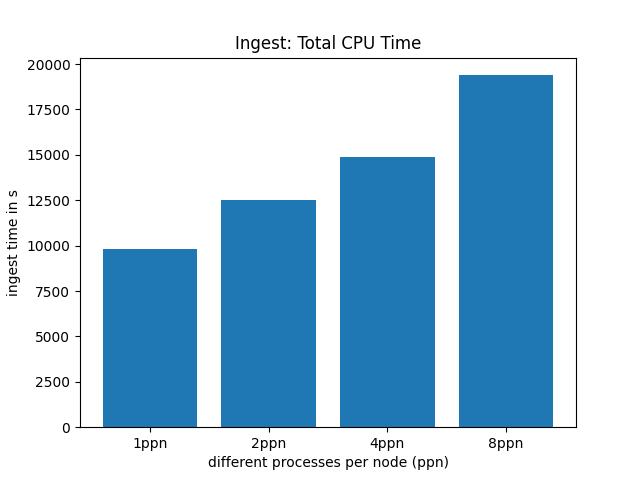
\includegraphics[width=0.45\textwidth]{./analysis/cputime.png} }}%
    \caption{Results showing wall clock time (a) (maximum execution time) and CPU time (b) (sum of all execution times) for different ppn.}%
\end{figure}

One can see that, as expected, by increasing the amount of load generators the wall clock time to ingest a given set of data decreases, although it unfortunately scales sublinear. But when looking at the CPU time, which is the sum of all wall clock times, the ingestion becomes more inefficient with more load generators. This is most likely due to the increased load on Elasticsearch, since the load generators themselves do not communicate between each other while ingesting, thus no additional MPI overhead should be measured.

\subsection{Queries}
The query benchmarks were also done for different ppn, here are some results based on the aforementioned range queries:

\begin{figure}[H]%
    \centering
    \subfloat[\centering {}]{{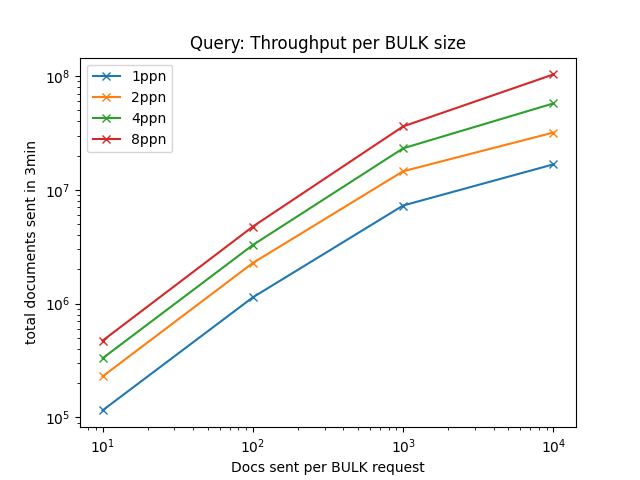
\includegraphics[width=0.45\textwidth]{./analysis/querythroughput.png} }}%
    \qquad
    \subfloat[\centering {}]{{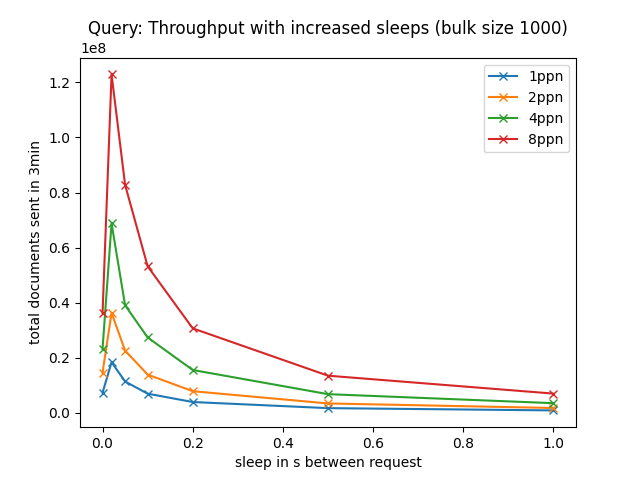
\includegraphics[width=0.45\textwidth]{./analysis/querythroughputsleep.png} }}%
    \caption{Scaling range queries along the BULK request size (a) (number of documents) and along the sleep between requests (b)}%
\end{figure}
The first plot shows scaling along the BULK request size. This means increasing the number of documents sent per request. It was measured in powers of 10, i.e. 10, 100, 1000, 10000 documents per request. The results are expected, since increasing the number of documents per request decreases the percentage wise network overhead, thus resulting in higher throughput. Furthermore it can be seen that it does not scale linearly\footnote{Note that both axis are logarithmic.} which shows that the Elasticsearch actually slows down from the increased overall load. More processes per node increase the throughput, implying that the server can still handle the number of processes well.\\

The second plot does the same query, but with increased waiting/sleep times off each load generator between the requests. Fascinatingly, it can be seen that a sleep time of $0.02s$ increases the throughput significantly over not sleeping at all. After that, it can be seen that increasing the sleep time decreases the overhead, which is to be expected since the nodes were not completely utilized while benchmarking.


\section{Challenges}
The design and implementation of the benchmarker still leaves two challenges open, both of which are not trivial to solve optimally.

\paragraph{Response Size:} If not specified otherwise, the Elasticsearch Search API will only return the 10 elements, even if more matching documents exist in the index. This number can be increased by the \texttt{size} parameter\footnote{\url{https://www.elastic.co/guide/en/elasticsearch/reference/current/paginate-search-results.html}}.

Unfortunately, due to performance reasons, this number can not be increased indefinitely. The maximum count of documents returnable by Elasticsearch is limited by the \texttt{index.max\_result\_window}\footnote{\url{https://www.elastic.co/guide/en/elasticsearch/reference/current/index-modules.html}} config setting, which defaults to 10000 documents. This means that only the first 10000 elements can be benchmarked. Theoretically, one can offset the result using the \texttt{from} parameter, practically Elasticsearch enforces the condition that \texttt{from+size <= index.max\_window}.\\

There are at least three solutions to this problem:
\begin{enumerate}
  \item Design the benchmarks around this constraint. For \texttt{nyc\_taxis}, this is what was done by Elastic; this is also the approach in most of the literature.
  \item Use the \texttt{search\_after} parameter for the search API\footnote{\url{https://www.elastic.co/guide/en/elasticsearch/reference/current/paginate-search-results.html\#search-after}}. This parameter takes the \texttt{sort} offset from a previous query and computes the new result starting from that offset.

    This approach has several big disadvantages. First, it blows up the complexity of both the benchmark design as well as the benchmarker logic by requiring statefulness between requests. The requests can't be done in a random manner since they always have to keep the offsets from previous responses. Additionally, it would make the benchmarking results harder to understand, as it may not be obvious how many requests were needed to get a specific amount of documents. Lastly, the \texttt{search\_after} parameter does not increase the complexity of each request, since it performs the same amount of work, except that it first seeks to a specific byte offset.

  \item Use this Scroll API\footnote{\url{https://www.elastic.co/guide/en/elasticsearch/reference/current/scroll-api.html}}. This has the same problem as the \texttt{search\_after} API as it requires keeping the state of a previous search query. Furthermore, according to Elastics documentation, its usage is discouraged for deep pagination of over 10000 elements.
\end{enumerate}

\paragraph{Load Generator to Cluster Node Mapping} As described in the methodology, each load generator sends its request to the same Elasticsearch cluster node every time. To provide roughly even load distribution, the node number is calculated by \texttt{MPI\_rank \% N} with \texttt{\%} being the modulo operation and \texttt{N} the number of Elasticsearch cluster nodes.

This node selection algorithm could result in a suboptimal usage of the network topology, resulting in longer package round trip times, for example requiring many hops in a fat tree structure.\\

\begin{figure}[H]
  \centering
  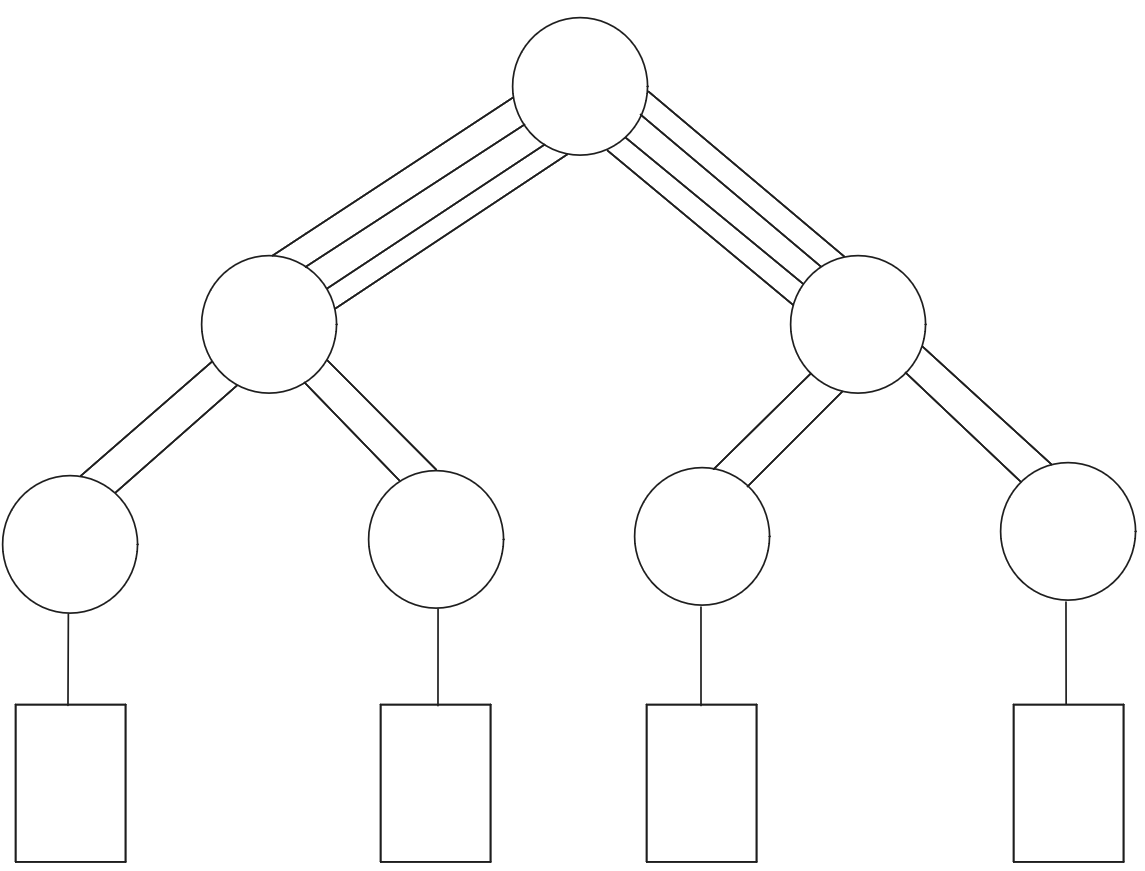
\includegraphics[width=0.7\textwidth]{./assets/fattree.png}
  \caption{An example of a fat tree. The leafs are nodes, and the intermediate nodes are routers. The higher the router, the more throughput it gets to provide to not limit the throughput by the higher degree nodes.}
\end{figure}


A possible solution would be to compute the optimal mapping every time before starting the benchmark. This could be done by measuring the round trip time between any pair of load generator and cluster node several times and using its mean or median average. Note that the lowest number can't always be used since all load generators have to be divided up onto the cluster nodes equally. Instead, this could be solved as a linear program\footnote{After some discussion with Johann Carl Meyer, who is a fellow student, I learned that this can be solved even more efficiently if seen as an optimal transport problem.}.\\

Unfortunately, this solution would overall worsen the benchmark results since, based on the current overall network usage, the routing could change between benchmarks, making the configuration indeterministic and thus the results unreproducible.

\section{Conclusion}
For the completion of this report, a zero-configuration workflow for automatically spawning and re-spawning a stateful Elasticsearch cluster was developed, allowing for job-based on-demand metadata processing as part of sophisticated job pipelines. Furthermore, a complete distributed benchmarking workflow was developed, including an ingestion benchmarker and a query benchmarker, allowing for large-scale benchmarks in \ac{HPC} environments. An example benchmark commonly used in the literature was successfully ported, executed, and analyzed. The code is fully accessible via GitHub, allowing it to be used as a platform for future performance research.

\subsection{Future Work}
As part of the data lake work at the GWDG, this benchmarker will be used to evaluate different encryption strategies based on their performance penalty. In general, most of the future work will be in the usage of the benchmarker for doing large-scale benchmarks, not in the extension of the benchmarker itself. 

As described in the Challenges, the primary open problem is figuring out how to handle response sizes larger than \texttt{index.max\_result\_window} through the methods above. Furthermore, currently it is not supported to run both the spawner and load generators on the same nodes, since the spawner is blocking the MPI environment. Lastly, a collection of common benchmarks that can be used for this benchmarker has to still be created over time.
